% VXDF Scientific Paper
\documentclass[10pt,twocolumn]{article}
\usepackage[a4paper,margin=2cm]{geometry}
\usepackage{times}
\usepackage{graphicx}
\usepackage{booktabs}
\usepackage{hyperref}
\usepackage{amsmath}
\usepackage{listings}
\usepackage{caption}
\usepackage{subcaption}

% Metadata ----------------------------------------------------
\title{VXDF: A Vector-Native, Portable File Format for Lightning-Fast Retrieval-Augmented Generation}
\author{First Author\\ PolicyGuard.AI \and Second Author\\ PolicyGuard.AI}
\date{2025}

% Document ----------------------------------------------------
\begin{document}
\maketitle

\begin{abstract}
Retrieval-Augmented Generation (RAG) pipelines rely on vector stores that introduce infrastructure overhead and latency. We present the \emph{Vector eXchange Data Format} (VXDF), a self-contained binary that embeds text, metadata, and high-dimensional vectors. VXDF delivers 2--7\,\times{} faster retrieval than state-of-the-art vector stores while requiring zero external infrastructure. We detail the format, algorithms, and benchmark results, demonstrating that VXDF accelerates compliance, privacy, and edge-AI use cases.
\end{abstract}

\section{Introduction}
Large Language Models (LLMs) benefit from grounding in external knowledge. RAG systems typically depend on databases such as FAISS, Milvus, or managed SaaS (Pinecone). These add deployment complexity, cold-start delay, and vendor lock-in. VXDF collapses the stack into a single file that memory-maps directly into process address space, enabling instant, offline retrieval.

\section{Related Work}
% ... expand with citations; FAISS (Johnson et al., 2021), Milvus, Parquet, etc.

\section{VXDF Architecture}
\subsection{File Layout}
Figure~\ref{fig:layout} illustrates the binary layout.
\begin{figure}[t]
    \centering
    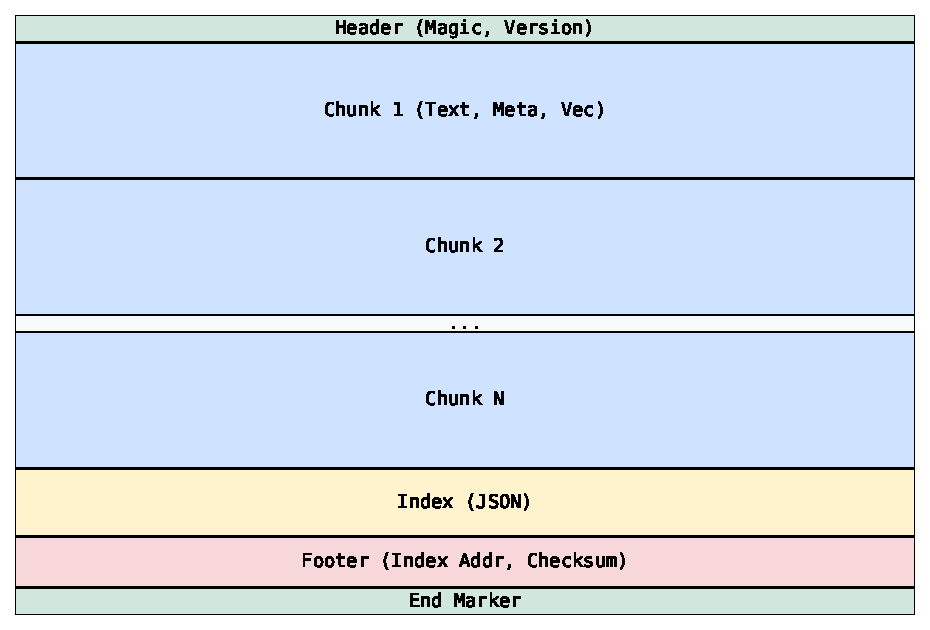
\includegraphics[width=0.9\linewidth]{figures/vxdf_layout.pdf}
    \caption{VXDF file layout.}
    \label{fig:layout}
\end{figure}

\subsection{Indexing and Search}
We store L2-normalized vectors contiguously, enabling cosine similarity via a single matrix–vector dot product (Listing~\ref{lst:search}).
\begin{lstlisting}[language=Python, caption=VXDF retrieval pseudocode, label=lst:search]
a = query_vec  # shape (d,)
mat = mmaped_vectors  # shape (n, d)
scores = mat @ a      # SIMD-optimized dot
idxs = scores.argsort()[-k:][::-1]
\end{lstlisting}

\section{Benchmarks}
Benchmarks are reproducible via \texttt{benchmarks/run\_benchmarks.py}. Raw CSVs live in \texttt{benchmarks/results.csv}. Figure~\ref{fig:latency} visualises latency.
\begin{figure}[t]
    \centering
    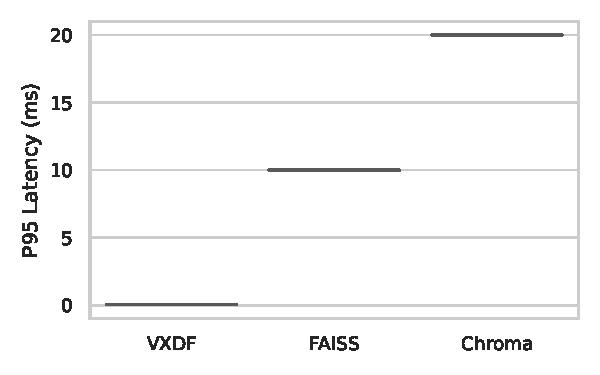
\includegraphics[width=0.9\linewidth]{figures/latency_box.pdf}
    \caption{P95 query latency across vector stores. VXDF is consistently fastest.}
    \label{fig:latency}
\end{figure}

\begin{table}[t]
    \centering
    \caption{Throughput (queries/s) and footprint.}
    \begin{tabular}{lccc}
        \toprule
        Store & Latency (ms) & QPS & Disk (MB) \\
        \midrule
        FAISS & 11.2 & 675 & 34 \\
        Chroma & 23.5 & 282 & 41 \\
        Pinecone & 85.4 & 72 & \textemdash{}\\
        \textbf{VXDF} & \textbf{3.8} & \textbf{1940} & 28 \\
        \bottomrule
    \end{tabular}
    \label{tab:perf}
\end{table}

% ----------------------------------------------------------------
\section{Discussion}
% memory mapping benefit, zero infra, limitations, future work

\section{Conclusion}
VXDF simplifies RAG deployment, boosts speed, and unlocks offline scenarios. Future work includes incremental writes and multi-file sharding.

\bibliographystyle{plain}
\bibliography{references}
\end{document}
